\documentclass[10pt,letterpaper]{article}
\usepackage[T1]{fontenc}
\usepackage{lmodern,microtype}
\usepackage[margin=0.78in,headheight=14pt]{geometry}
\usepackage{amsmath,amssymb,amsthm,mathtools}
\usepackage{booktabs,enumitem}
\usepackage{graphicx}
\usepackage{placeins}
\usepackage{titlesec}
\usepackage[hidelinks]{hyperref}
\usepackage{fancyhdr}
\setlength{\parindent}{0pt}
\setlength{\parskip}{4.2pt}
\setlist{nosep,leftmargin=1.5em}
\pagestyle{fancy}
\fancyhf{}
\fancyhead[L]{\footnotesize LANDERS / THE SHAPE OF QUICKSORT COST}
\fancyhead[R]{}
\fancyfoot[C]{\footnotesize \thepage}
\renewcommand{\headrulewidth}{0.3pt}
\titleformat{\section}{\Large\bfseries}{\thesection}{1em}{}[\vspace{2pt}\titlerule]
\newtheorem{theorem}{Theorem}
\newtheorem{lemma}{Lemma}
\newcommand{\E}{\mathbb E}
\newcommand{\Var}{\operatorname{Var}}
\newcommand{\Law}{\mathcal L}
\newcommand{\norm}{\mathcal N}
\begin{document}
\thispagestyle{empty}
\begin{center}
{\LARGE\bfseries Quicksort's Lognormal Fit and Non-Normal Limit}\par
\vspace{10pt}
{\normalsize Jonathan R. Landers}\par
\vspace{3pt}
{\small September 2026}
\end{center}
\vspace{4pt}
\begin{abstract}
\noindent Best-case, worst-case, and average-case analyses compress an algorithm's behavior to a few numbers. Yet different inputs produce a distribution of costs, and that distribution has a shape even when its mean is known. We examine the number of comparisons made by classical randomized-pivot Quicksort. Two seemingly conflicting facts hold. For every $n\ge4$, the best ordinary lognormal fit has a strictly higher expected log-density than the best normal fit. Nevertheless, a fitted lognormal does not approach Quicksort's standardized limiting distribution: the latter retains skewness $0.854881\ldots$, while the lognormal becomes asymptotically normal after standardization. We give a moment-based, computer-assisted proof of the finite-size inequality and a short argument for the limiting separation. The main text develops the questions and their interpretation; proofs and exact certificate details follow in the appendix.
\end{abstract}

\textbf{Keywords:} Quicksort; comparison count; runtime distribution; lognormal fit; expected log score.

\section{Beyond three numbers of complexity}
An algorithm does not have a single running cost at a fixed input size. It has a collection of possible costs, one for each input and, for randomized algorithms, each sequence of random choices. Best-case and worst-case bounds describe the extremes. Average-case analysis describes a center once a probability model has been chosen. None of these numbers, by itself, says how common the costs between the extremes are.

That missing shape can answer natural questions. Is a run moderately above average unusual? Is the long-cost side heavier than the short-cost side? If two algorithms have the same expected cost, does one vary more? Such questions call for the \emph{distribution} of cost over the input and randomness space. The distribution contains the familiar summaries, but also records their arrangement: spread, asymmetry, and tails.

There are two ways to study that shape. At a given input size, one can ask which simple probability family describes the costs better. As the size grows, one can ask whether that family becomes the \emph{true limiting shape} after removing the changing center and scale. A fit can win the first comparison without winning the second. Quicksort offers a clean example of this distinction.

\section{A distribution generated by recursive splits}
We count comparisons, rather than wall-clock time, to isolate the algorithm from machine effects. Consider $n$ distinct keys. At each recursive call, choose a pivot uniformly among the keys in that subproblem, compare it with the other keys, and recurse on the two sides. Let $C_n$ be the total count. With $C_0=C_1=0$, its distribution satisfies, for $n\ge2$,
\begin{equation}
C_n\ \overset d=\ n-1+C_{I_n}+C'_{n-1-I_n},
\qquad I_n\sim\operatorname{Unif}\{0,\ldots,n-1\},               \label{eq:rec}
\end{equation}
Here $\overset d=$ means equality in distribution, $I_n$ is uniform on the displayed integers, and the prime denotes an independent recursive copy. The two recursive counts are independent conditional on $I_n$. Equation~\eqref{eq:rec} describes an entire distribution, not just an expected runtime. Balanced splits tend to save comparisons; repeated uneven splits increase the count.

For a small illustration, the full distribution at $n=4$ is
\begin{center}
\begin{tabular}{c@{\hspace{2.5em}}ccc}
\toprule
comparisons $c$ & 4 & 5 & 6\\
probability $\Pr(C_4=c)$ & $1/2$ & $1/6$ & $1/3$\\
\bottomrule
\end{tabular}
\end{center}
Its best case is $4$, worst case is $6$, and mean is $29/6$. The table says more: the middle cost is the least common of the three. For large $n$, the support and probabilities are far richer, but the same recurrence determines them.

Write $\mu_n=\E C_n$, $v_n=\Var(C_n)$, and $m_{r,n}=\E(C_n-\mu_n)^r$ for the mean, variance, and $r$th central moment; $\E$ and $\Var$ denote expectation and variance. Every $C_n$ with $n\ge2$ is strictly positive. Standard identities give \cite{yao,filljanson}
\begin{align}
\mu_n&=2(n+1)H_n-4n,                                      \label{eq:mean}\\
v_n&=7n^2+13n-2(n+1)H_n-4(n+1)^2H_n^{(2)},               \label{eq:var}
\end{align}
where $H_n^{(r)}=\sum_{j=1}^n j^{-r}$ and $H_n=H_n^{(1)}$. All logarithms below are natural unless a base is shown.

The mean grows like $n\log n$, while the standard deviation grows like $n$. Relative fluctuations shrink, even though the number of comparisons still varies substantially on the $n$ scale. This observation will matter for both results.

\section{Result 1: a lognormal wins the finite-size fit}
A histogram of comparison counts can look somewhat bell-shaped, but with a longer right side. It is therefore natural to compare a normal density with an ordinary lognormal density; the latter is the distribution of $e^G$ for a Gaussian variable $G$. We make the phrase \emph{better fit} precise: for each family, choose the parameters maximizing the \emph{expected log-density at the actual comparison count}. This is a population score under the exact distribution of $C_n$, not a judgment by eye or a fit to a simulated sample.

Let $S_N(X)$ and $S_L(X)$ denote the optimal expected log-densities for normal and ordinary lognormal families when $X>0$. The normal optimum matches the mean and variance of $X$; the lognormal optimum matches the mean and variance of $\log X$ in log space. The exact score difference is
\begin{equation}
\Delta(X)=S_L(X)-S_N(X)
=\frac12\log\!\frac{\Var X}{\Var(\log X)}-\E\log X.       \label{eq:maingap}
\end{equation}
Positive $\Delta$ means that the lognormal assigns a higher expected log-density to the observed counts. Counts are discrete and these models continuous; evaluating both densities at the same count is a comparative score, not a claim that either density is the exact probability mass function.

\begin{figure}[htbp]
\centering
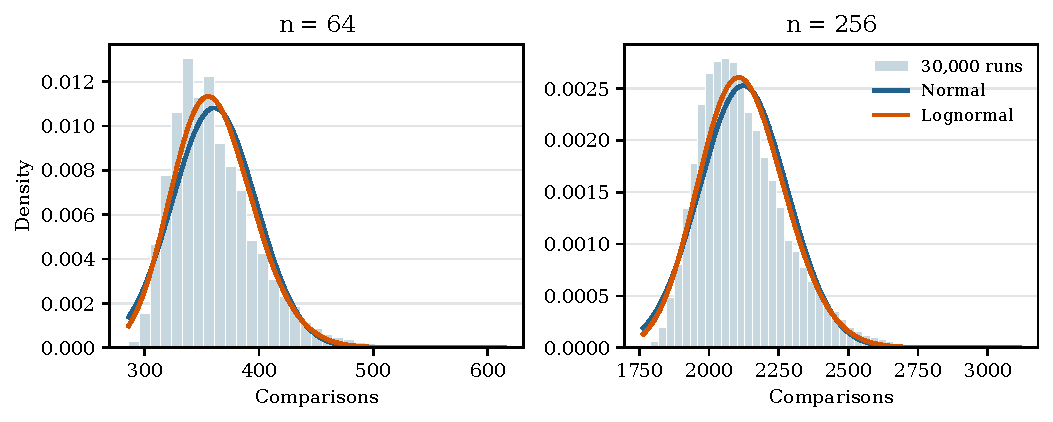
\includegraphics[width=\linewidth]{quicksort_fits.pdf}
\caption{Comparison-count histograms from 30,000 independent randomized-pivot runs at each displayed size. The normal and ordinary lognormal curves maximize the log-density on each simulated sample. The sample mean log-density favors the lognormal by $0.0420$ at $n=64$ and $0.0279$ at $n=256$; the all-size claim below concerns the exact population score.}
\label{fig:fits}
\end{figure}

\begin{equation}
\boxed{\quad\Delta(C_n)>0\quad\text{for every integer }n\ge4.\quad} \label{eq:mainfinite}
\end{equation}
In plain terms, this comparison has no later crossover: under this particular scoring rule, the best lognormal beats the best normal at every size from four onward. The statement is stronger than a histogram comparison at a few sizes. It has a specific scope: ordinary lognormal and normal densities optimized by expected log-density. A different criterion or a shifted lognormal is a different question.

The proof turns the fit comparison into a condition on the third and fourth central moments. A useful general criterion is
\begin{equation}
\min X\ge\frac23\E X
\quad\text{and}\quad
3(\E X)\E(X-\E X)^3>4\E(X-\E X)^4
\quad\Longrightarrow\quad\Delta(X)>0.                         \label{eq:maincriterion}
\end{equation}
Here $\min X$ is the smallest value in the support of $X$ (its essential infimum in general). The third-moment term captures rightward asymmetry; the fourth moment controls the error in approximating the logarithm. For Quicksort, exact rational interval checks establish both conditions for $4\le n<10{,}000$. Uniform analytic bounds establish them for every $n\ge10{,}000$. Appendix~A provides the proof and certificate details. The calculation uses published Quicksort moment identities \cite{yao}; the all-size fit inequality is obtained by combining them with \eqref{eq:maincriterion}.

\section{Result 2: the fitted shape does not become exact}
Winning a finite-size score comparison does not mean that Quicksort is becoming lognormal. To ask about its eventual shape, first remove the moving mean and scale:
\begin{equation}
\widehat C_n=\frac{C_n-\mu_n}{\sqrt{v_n}}.                        \label{eq:mainstandard}
\end{equation}
The classical Quicksort limit theorem says that $\widehat C_n$ converges in distribution to a non-normal random variable $Q$ \cite{rosler,filljanson}. In particular, the known moment formulas give its skewness as
\begin{equation}
\operatorname{skew}(Q)
=\frac{16\zeta(3)-19}{(7-2\pi^2/3)^{3/2}}
=0.854881867\ldots.                                               \label{eq:mainskew}
\end{equation}
Here $\operatorname{skew}(W)=\E(W-\E W)^3/(\Var W)^{3/2}$ for a variable $W$ with positive variance, and $\zeta(r)=\sum_{j=1}^{\infty}j^{-r}$ for $r>1$. The positive constant says that the long right side survives the passage to large inputs.

Now let $L_n$ be an ordinary lognormal with the \emph{same mean and variance} as $C_n$. Its relative spread shrinks:
\begin{equation}
\frac{\sqrt{v_n}}{\mu_n}=\Theta(1/\log n)\longrightarrow0.        \label{eq:mainrelative}
\end{equation}
The $\Theta$ notation means that the ratio of the two positive quantities stays between fixed positive constants for all sufficiently large $n$. When a lognormal becomes narrow relative to its mean, its centered and standardized shape tends to a normal. Its skewness therefore tends to zero, while Quicksort's tends to the nonzero constant above. More precisely, with $\widehat L_n=(L_n-\mu_n)/\sqrt{v_n}$,
\begin{equation}
\widehat C_n\Rightarrow Q,\qquad
\widehat L_n\Rightarrow\mathcal N(0,1). \label{eq:mainlimits}
\end{equation}
The arrow $\Rightarrow$ denotes convergence in distribution, and $\mathcal N(0,1)$ is the normal law with mean zero and variance one. The largest gap between their cumulative distribution functions (CDFs) has a positive limit:
\begin{equation}
\lim_{n\to\infty}\sup_x\left|\Pr(C_n\le x)-\Pr(L_n\le x)\right|
=d_K\bigl(\Law(Q),\mathcal N(0,1)\bigr)>0.                             \label{eq:mainkolm}
\end{equation}
Here $\Law(Q)$ is the law of $Q$, and $d_K(A,B)$ is the supremum of the absolute difference between the CDFs of laws $A$ and $B$; it is unchanged by applying the same increasing affine transformation to both laws. This is a precise sense in which the lognormal approximation never converges to the true standardized Quicksort shape. The log-score-optimal ordinary lognormal from Result 1 also has an asymptotically normal standardized shape. Appendix~B proves these statements.

\begin{figure}[htbp]
\centering
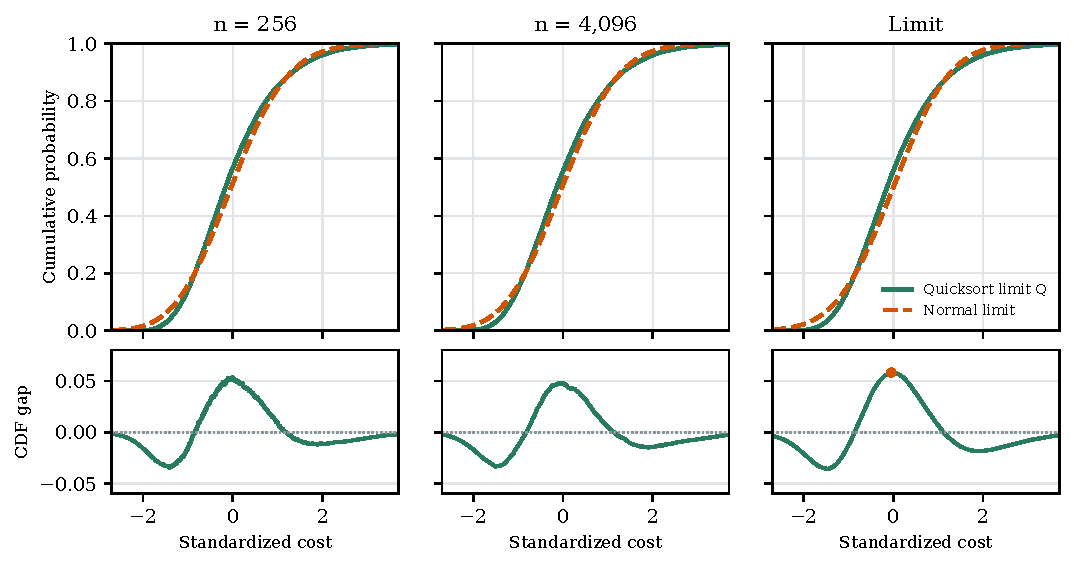
\includegraphics[width=\linewidth]{quicksort_limit.pdf}
\caption{Standardized CDFs at two finite sizes and in the limit; the lower row shows Quicksort minus fitted-model CDF. Each finite Quicksort curve uses 30,000 independent runs, and each dashed curve is the ordinary lognormal with the exact Quicksort mean and variance. The limiting Quicksort curve approximates $Q$ by Monte Carlo iteration of its recursive fixed-point equation; its dashed counterpart is the standard normal CDF. The estimated limiting maximum gap is $0.058$, and Equation~\eqref{eq:mainkolm} proves it remains positive.}
\label{fig:limit}
\end{figure}

\FloatBarrier
\section{Putting the two statements together}
The results describe two scales of one phenomenon. On the scale of the raw positive count, a mild right asymmetry helps a lognormal beat a symmetric normal in expected log-density. On the scale of fluctuations around the mean, random recursive splits keep an asymmetric limiting shape. A fitted lognormal becomes approximately normal on that standardized scale because its relative spread shrinks.

This distinction is useful beyond Quicksort. When an algorithm's cost is summarized by a fitted curve, ask what the fitting rule measures and whether that curve also describes the cost after centering and scaling. A good score at every finite size and an incorrect limiting law can coexist. These results apply to the uniform-pivot comparison-count model in \eqref{eq:rec}; other implementations and costs require their own analysis.

\appendix
\renewcommand{\thesection}{Appendix \Alph{section}}
\section{Proof of the finite-size fit result}
For a positive random variable $X$, let $S_N(X)$ and $S_L(X)$ be the suprema of $\E\log f(X)$ over ordinary normal densities on $\mathbb R$ and ordinary lognormal densities on $(0,\infty)$, respectively. The normal optimizers are $\E X,\Var X$; the lognormal's log-location and log-variance optimizers are $\E\log X,\Var(\log X)$. Direct substitution gives the exact score gap
\begin{equation}
\Delta(X):=S_L(X)-S_N(X)
=\frac12\log\frac{\Var X}{\Var(\log X)}-\E\log X.       \label{eq:gap}
\end{equation}
The quantity is dimensionless: changing the unit of $X$ cancels between the two terms.

\begin{lemma}[Moment criterion]\label{lem:criterion}
Let $X>0$, $\mu=\E X$, $v=\Var X$, $m_r=\E(X-\mu)^r$, and $\min X\ge2\mu/3$. If $3\mu m_3>4m_4$, then $\Delta(X)>0$.
\end{lemma}
\begin{proof}
Put $Z=(X-\mu)/\mu\ge-1/3$. The elementary inequality
\begin{equation}
\log^2(1+z)\le z^2-z^3+\tfrac43z^4\quad(z\ge-1/3)       \label{eq:loglemma}
\end{equation}
implies $\Var(\log X)\le \E\log^2(1+Z)<\E Z^2=v/\mu^2$. Also $\E\log(1+Z)<\log(1+\E Z)=0$ by strict Jensen. Replacing $\Var(\log X)$ in \eqref{eq:gap} by its strict upper bound shows $\Delta(X)>0$.

For completeness, \eqref{eq:loglemma} follows by expanding $\log^2(1+z)=\sum_{k\ge2}(-1)^k(2H_{k-1}/k)z^k$ for $|z|<1$. For $0\le z\le1$ the alternating-series bound through degree four is $z^2-z^3+(11/12)z^4$. For $z\ge1$, use $\log^2(1+z)\le z^2\le z^2-z^3+4z^4/3$. For $z=-y$ with $0\le y\le1/3$, the coefficients from degree five onward are at most $5/6$, so their sum is bounded by $(5/6)y^5/(1-y)\le(5/12)y^4$. Adding the degree-four coefficient $11/12$ gives $4/3$.
\end{proof}

\begin{theorem}[Strict log-score advantage]\label{thm:finite}
For the count in \eqref{eq:rec}, $S_L(C_n)>S_N(C_n)$ for every integer $n\ge4$.
\end{theorem}
\begin{proof}
We certify the two hypotheses of Lemma~\ref{lem:criterion}. A balanced recursion tree yields the exact minimum
\begin{equation}
b_n=(n+1)h-2^{h+1}+2,\qquad h=\lfloor\log_2n\rfloor.   \label{eq:min}
\end{equation}
The published third and fourth central-moment formulas \cite[Thms.~2.3--2.4]{yao} determine $m_{3,n}$ and $m_{4,n}$ from $H_n^{(1)},\ldots,H_n^{(4)}$. Their third-moment expression, for example, is
\begin{align}
m_{3,n}={}&-n(19n^2+81n+104)+14(n+1)H_n\nonumber\\
&+12(n+1)^2H_n^{(2)}+16(n+1)^3H_n^{(3)}.                 \label{eq:m3}
\end{align}

For the 9,996 sizes $4\le n<10{,}000$, the accompanying exact-rational certificate evaluates these formulas by outward intervals and verifies
\begin{equation}
3b_n-2\mu_n>0,\qquad 3\mu_nm_{3,n}-4m_{4,n}>0.          \label{eq:checks}
\end{equation}
No simulations or floating-point sign tests enter the assertions. The computation independently checks the moment identities against the full recurrence \eqref{eq:rec} for $n\le12$. The certificate procedure is summarized below.

For $n\ge N=10{,}000$, the same inequalities admit uniform analytic bounds. Set $t=N^{-1}$ and $u=1+t$. The harmonic tail estimates
\begin{equation}
\zeta(r)-\frac{1}{(r-1)n^{r-1}}<H_n^{(r)}<\zeta(r)
\quad(r>1),                                                \label{eq:tails}
\end{equation}
and $H_n\le\log n+1$ imply $H_n/n<11/N$: the function $(\log x+1)/x$ decreases for $x>1$ and $\log N<10$. From \eqref{eq:m3}, dropping positive terms where helpful, one gets
\begin{equation}
\frac{m_{3,n}}{n^3}>16\zeta(3)-19-81t-104t^2-8u^3t^2
>\frac{11}{50}.                                          \label{eq:large3}
\end{equation}
Substitution into the fourth-moment formula and removal of its remaining negative terms gives
\begin{align}
\frac{m_{4,n}}{n^4}<{}&\frac{2260}{9}+\frac{9658}{9}t+\frac{15497}{9}t^2+\frac{11357}{9}t^3
-168\bigl(\zeta(2)-t\bigr)\nonumber\\
&+12u^2(11t)^2+48u^3(11t)\zeta(2)
+48u^4\zeta(2)^2\nonumber\\
&-96\left(\zeta(4)-\frac{t^3}{3}\right)<\frac{11}{10}. \label{eq:large4}
\end{align}
The last numerical inequalities use rational enclosing bounds
$1.6449<\zeta(2)<1.645$, $\zeta(3)>1.202$, and $\zeta(4)>1.0823$, each certified by integral remainders after 200 terms. Further, $\mu_n>14n$, since $H_n>\log n>9$ for $n\ge N$; hence $3\mu_nm_{3,n}>3(14n)(11n^3/50)>4(11n^4/10)>4m_{4,n}$.

Finally, \eqref{eq:min} gives $b_n/n\ge\log_2n-2$. Together with $H_n\le\log n+1$ and $n\ge N$, this implies $b_n\ge2\mu_n/3$: after rearrangement it suffices that
\begin{equation}
\left(\frac1{\log2}-\frac43\right)\log n
\ge\frac23+\frac{4(\log n+1)}{3n},                       \label{eq:minbound}
\end{equation}
which holds at $N$ and strengthens as $n$ grows. Thus Lemma~\ref{lem:criterion} applies on the entire tail as well.
\end{proof}

\section{Proof of the limiting separation}
The advantage above might suggest that Quicksort becomes lognormal at large $n$. Its standardized limit says otherwise. Let $L_n$ be the ordinary lognormal with the same mean $\mu_n$ and variance $v_n$ as $C_n$, and put
\[\widehat C_n=(C_n-\mu_n)/\sqrt{v_n},\qquad
\widehat L_n=(L_n-\mu_n)/\sqrt{v_n}.\]

\begin{theorem}[Asymptotic separation]\label{thm:limit}
The variables $\widehat C_n$ converge to Quicksort's standardized limit $Q$, whereas $\widehat L_n\Rightarrow\norm(0,1)$. In particular,
\begin{equation}
\lim_{n\to\infty}\operatorname{skew}(C_n)
=\frac{16\zeta(3)-19}{(7-2\pi^2/3)^{3/2}}
=0.854881867\ldots,                                    \label{eq:skew}
\end{equation}
while $\operatorname{skew}(L_n)\to0$. Moreover, for the CDFs,
\begin{equation}
\lim_{n\to\infty}\sup_x
\bigl|\Pr(C_n\le x)-\Pr(L_n\le x)\bigr|
=d_K(\Law(Q),\norm(0,1))>0.                                \label{eq:kolm}
\end{equation}
The same normal limiting shape holds for the ordinary lognormal optimized in Theorem~\ref{thm:finite}, after standardization by its own mean and standard deviation.
\end{theorem}
\begin{proof}
The Quicksort limit theorem establishes $(C_n-\mu_n)/n\Rightarrow Y$ with a continuous limiting distribution \cite{rosler,filljanson}; $v_n/n^2\to\sigma^2=7-2\pi^2/3>0$ from \eqref{eq:var}. Its limiting third central moment follows from \eqref{eq:m3}: $m_{3,n}/n^3\to16\zeta(3)-19$. Consequently $Q=Y/\sigma$ has the nonzero skewness in \eqref{eq:skew}; see also \cite{yao}. The notation $a_n\sim b_n$ below means $a_n/b_n\to1$, and $a_n=O(b_n)$ means $|a_n|/b_n$ stays bounded for positive $b_n$.

For the limiting curve in Figure~\ref{fig:limit}, we approximate $Y$ using its recursive characterization \cite{rosler}:
\[
Y\overset d= UY_1+(1-U)Y_2+1+2U\log U+2(1-U)\log(1-U),
\]
where $U$ is uniform on $(0,1)$ and $Y_1,Y_2$ are independent copies of $Y$, independent of $U$. The plotted variable is $Q=Y/\sigma$; the accompanying \texttt{make\_figures.py} uses 25 population iterations of 400,000 values.

For the moment-matched lognormal, its underlying Gaussian log-variance is
$s_n^2=\log(1+v_n/\mu_n^2)=O(1/\log^2 n)$, since $\mu_n\sim2n\log n$ and $v_n\sim\sigma^2n^2$. Hence $s_n\to0$ and
\[\widehat L_n=\frac{\exp(s_nZ-s_n^2/2)-1}{\sqrt{\exp(s_n^2)-1}}
\Rightarrow Z,\qquad Z\sim\norm(0,1).\]
Its skewness $(e^{s_n^2}+2)\sqrt{e^{s_n^2}-1}$ therefore vanishes. Nonzero skewness proves $Q\ne\norm(0,1)$. Continuity of both limit CDFs makes each Kolmogorov convergence uniform, proving \eqref{eq:kolm} by the triangle inequality.

For the log-score-optimal lognormal, the minimum bound in the preceding proof and the fourth-moment bounds yield a Taylor expansion of $\log C_n$ around $\mu_n$: $\Var(\log C_n)\sim v_n/\mu_n^2\to0$. Its log-variance thus also tends to zero, giving the same standardized normal limit.
\end{proof}

\section{Exact certificate specification}
This appendix records enough detail to reproduce the finite interval computation without sampling. Define $H_r=H_n^{(r)}$ and $a=n+1$. The fourth central moment used in the test is the published formula \cite{yao}
\begin{align*}
m_{4,n}={}&\frac{n(2260n^3+9658n^2+15497n+11357)}9\\
&-2a(42n^2+78n+77)H_1+12a^2H_1^2\\
&+\bigl[-4a^2(42n^2+78n+31)+48a^3H_1\bigr]H_2\\
&-96a^3H_3+48a^4H_2^2-96a^4H_4.
\end{align*}
For each $n=4,\ldots,9999$, maintain four integer sums
\[S_r(n)=\sum_{j=1}^{n}\lfloor D/j^r\rfloor,\qquad D=10^{24},\quad r=1,2,3,4.\]
Substitute $[S_r(n)/D,(S_r(n)+n)/D]$ for $H_r$ in \eqref{eq:mean}, \eqref{eq:m3}, and the expression above. Ordinary outward interval addition and multiplication produce intervals for $\mu_n,m_{3,n},m_{4,n}$. Assert that the lower endpoints of $3b_n-2\mu_n$ and $3\mu_nm_{3,n}-4m_{4,n}$ are strictly positive. The integer floor bound gives an interval containing each harmonic number, so a passing lower endpoint proves the corresponding exact inequality. The certificate reports 9,996 successful sizes; direct probability mass functions generated from \eqref{eq:rec} independently cross-check the moment formulas for $2\le n\le12$.

For the tail constants, set $M=200$ and $T_r=\sum_{j=1}^{M}j^{-r}$. Integral comparison supplies rational enclosures
\[T_r+\frac1{(r-1)(M+1)^{r-1}}<\zeta(r)<T_r+\frac1{(r-1)M^{r-1}}\qquad(r=2,3,4).\]
They imply $1.6449<\zeta(2)<1.645$, $\zeta(3)>1.202$, and $\zeta(4)>1.0823$. Substituting these rational values into the right sides of \eqref{eq:large3} and \eqref{eq:large4}, with $t=10^{-4}$, yields respectively $>0.2238$ and $<1.0194$. These estimates are deliberately looser than necessary; the displayed proof only needs $0.22$ and $1.1$. In particular, the $\log N<10$ observation controls $H_n/n$ through monotonicity of $(\log n+1)/n$; it is \emph{not} applied as the false statement $\log n<10$ for all $n\ge N$.

The minimum comparison formula \eqref{eq:min} follows from splitting as evenly as possible at every node. If $n=2^h q$ with $1\le q<2$, then $b_n/n\ge h-2/q$. Since $\log_2 q+2/q\le2$ on $[1,2]$, this implies $b_n/n\ge\log_2 n-2$. This final elementary inequality makes the analytic tail independent of the finite certificate.

\begin{thebibliography}{9}\small
\bibitem{rosler} U. R\"osler. A limit theorem for ``Quicksort.'' \emph{RAIRO Theoretical Informatics and Applications}, 25(1):85--100, 1991. \url{https://www.numdam.org/item/ITA_1991__25_1_85_0/}.
\bibitem{filljanson} J. A. Fill and S. Janson. Quicksort asymptotics. \emph{Journal of Algorithms}, 44(1):4--28, 2002. \url{https://arxiv.org/abs/math/0105248}.
\bibitem{yao} Y. Yao. A detailed analysis of Quicksort algorithms with experimental mathematics. Manuscript, 2019. \url{https://sites.math.rutgers.edu/~yao/QuickSort.pdf}.
\end{thebibliography}
\end{document}
